\documentclass[czech]{beamer}
\usetheme{m}
%\usepackage[T1]{fontenc}
%\usepackage[utf8]{inputenc}
\usepackage{babel}
\newtheorem{priklad}{Příklad}
\newtheorem{pozor}{Pozor!}
\addtobeamertemplate{block begin}{\setlength\abovedisplayskip{0pt}}{}
\addtobeamertemplate{block end}{\vspace*{-1em}}{}


\newcommand\myfig[3][width=.9\textwidth]{%
  \figure\includegraphics[#1]{#2}%
  \caption{#3}%
\endfigure}

\usepackage{graphicx}
\title{Tvorba elektronických knih systémem tex4ebook}
\author{Michal Hoftich\inst{1}}
\institute{
  \inst{1}
  <\url{michal.h21@gmail.com}>\\
  Ústřední knihovna PedF UK
}

\date{Přednáška pro CSTUG 2015}

\begin{document}

\frame{\titlepage}

\begin{frame}
  \frametitle{Obsah}
  \tableofcontents
\end{frame}

\section{Formáty elektronických knih}
\begin{frame}
\frametitle{Podporované formáty elektronických knih}
  \begin{itemize}%[<+->]
\item ePUB 
  \begin{itemize}
    \item nejrozšířenější podpora ve čtečkách
    \item některé nepodporují ani kaskádové styly
  \end{itemize}
\item mobi
  \begin{itemize}
    \item podpora ve čtečkách Kindle od Amazonu
    \item vzniká konverzí z ePUBu programem kindlegen
  \end{itemize}
\item ePUB3
\end{itemize}
\end{frame}
\begin{frame}
  \frametitle{Nové možnosti v ePUB3}
  \begin{itemize}%[<+->]
    \item Nové standardy
      \begin{itemize}
    \item  html5
    \item  mathml
    \item  CSS 3
    \item  SMIL
    \item  SVG
  \end{itemize}
  \end{itemize}
\end{frame}
\begin{frame}
  \frametitle{Nové možnosti v ePUB3}
  \begin{itemize}%[<+->]
    \item fixed layout
    \item  javascript
      \begin{itemize}
        \item  interaktivní prvky
        \item vylepšení dokumentu
      \end{itemize}
    \item  struktura dokumentu
      \begin{itemize}
        \item  (frontmatter, mainmatter, backmatter)
        \item  dělení dokumentu (volume, part, chapter, subchapter)
      \end{itemize}
    \item logické značkování
      \begin{itemize}
        \item rejstříky
        \item slovníky
      \end{itemize}
     \item profily
       \begin{itemize}
     \item edupub
   \end{itemize}
\end{itemize}
\end{frame}
\begin{frame}
        \frametitle{Příklad: Calzone }
\url{https://github.com/michal-h21/calzone}
\begin{figure}
  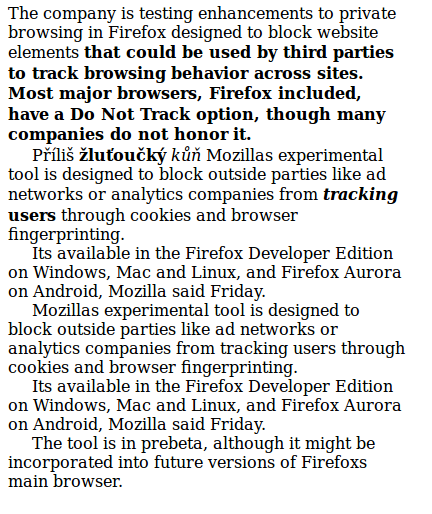
\includegraphics[width=.6\textwidth]{examples/without-calzone.png}
  \caption{Normální odstavec zarovnaný do bloku, tak jak ho zobrazí prohlížeč}
\end{figure}
\end{frame}
\begin{frame}
        \frametitle{Příklad: Calzone }
\url{https://github.com/michal-h21/calzone}
\begin{figure}
  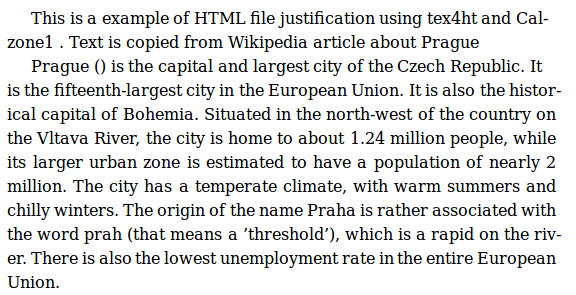
\includegraphics[width=.6\textwidth]{examples/with-calzone.png}
  \caption{Zalomení odstavce s \texttt{calzone.js}}
  \end{figure}
\end{frame}
\begin{frame}
  \frametitle{Javascript v ePUB}
\begin{pozor}
        Platí zásada, že dokument musí být použitelný i ve čtečce bez podpory JS
      \end{pozor}
\end{frame}
\begin{frame}
  \frametitle{Čtecí aplikace pro ePUB 3}
  \begin{itemize}
  \item čtečky s e-inkem ho prakticky nepodporují
  \item iBooks
  \item Adobe Digital Editions
  \item Android - Gitden
  \item Azardi
  \item Readium SDK
  \item Menestrello
\end{itemize}
\end{frame}
\begin{frame}
  \frametitle{Validace}
  \begin{itemize}
    \item pro validaci existuje nástroj ePUBcheck
    \item \url{https://github.com/IDPF/epubcheck}
  \end{itemize}
\end{frame}
\begin{frame}
  \frametitle{Příklad: Zobrazení matematiky}
  {\myfig{examples/png-epub.png}{Matematika ve formátu PNG. Azardi}}
\end{frame}
\begin{frame}
  \frametitle{Příklad: Zobrazení matematiky}
  {\myfig{examples/png-mobi.png}{Matematika ve formátu PNG. Kindle}}
\end{frame}
\begin{frame}
  \frametitle{Příklad: Zobrazení matematiky}
  \myfig{examples/svg-epub.png}{Matematika ve formátu SVG. Azardi}
\end{frame}
\begin{frame}
  \frametitle{Příklad: Zobrazení matematiky}
  \myfig[height=0.6\paperheight]{examples/svg-mobi.png}{Matematika ve formátu SVG. Kindle}
\end{frame}
\begin{frame}
  \frametitle{Příklad: Zobrazení matematiky}
  \myfig{examples/mathml-ade.png}{Matematika ve formátu MathML. ADE}
\end{frame}

  \section{Systém tex4ht}
\begin{frame}
  \frametitle{Historie tex4ht}
  \begin{itemize}
    \item \url{https://www.tug.org/tex4ht/}
    \item původní autor Eitan Gurari (1947--2009)
    \item systém vzniká od poloviny 90. let
    \item po smrti původního autora se o vývoj starají Karl Berry, CV Radhakrishnan a Michal Hoftich
  \end{itemize}
\end{frame}

\begin{frame}
  \frametitle{Další konvertory do HTML}
  \begin{itemize}
    \item Pandoc
    \item LaTeXML
    \item LaTeX2HTML
  \end{itemize}
\end{frame}

\begin{frame}

  \frametitle{Základní popis systému}
  \begin{itemize}
    \item systém se skládá z množství kompilačních skriptů, které se ale liší
      jen v přednastavených hodnotách
  \item základní skript je \texttt{htlatex} 
  \item například pro konverzi do ODT slouží \texttt{mk4ht oolatex}
  \item kompilace sestává ze tří základních kroků:
\end{itemize}
\end{frame}
\begin{frame}
  \frametitle{kompilace dokumentu TeXem s nahraným souborem tex4ht.sty}
  \begin{itemize}
    \item pro podporované balíčky jsou nahrané \texttt{.4ht} soubory, které vkládají
        konfigurovatelné háčky na vhodná místa
    \item po vložení háčků se nahrají jejich konfigurace v závislosti na
        výstupním formátu
  \end{itemize}
\end{frame}
\begin{frame}
  \frametitle{Zpracování dvi souboru programem tex4ht}
  \begin{itemize}
    \item   zápis výstupních souborů
    \item   konverze znakových sad
      \begin{itemize} 
        \item  poměrně komplikovaný proces, potřebujeme
          doplňkové soubory pro fonty obsahující unicode entity nebo ASCII
          znaky pro jednotlivé znaky písma
  \end{itemize}
    \item   zachovává základní styly písem, podporuje jakákoli makra měnící vzhled písma
    \item   příprava .lg souboru
    \item   zápis .idv souboru obsahující stránky pro konverzi na obrázky
  \end{itemize}
\end{frame}
\begin{frame}
  \frametitle{Zpracování .lg souboru programem t4ht}
  \begin{itemize}
    \item   výstup do CSS souboru
    \item   konverze vložených obrázků z .dvi do výstupního formátu
    \item   zpracování výstupních souborů externími programy 
    (\texttt{xslt}, \texttt{tidy}, \texttt{xmllint}, \texttt{xtpipes})
    \item   kopírování souborů do cílového adresáře
  \end{itemize}
\end{frame}
\begin{frame}[fragile]
  \frametitle{Kompilační skripty}
  \begin{itemize}
    \item parametry pro každý jednotlivý krok se předávají kompilačnímu skriptu v závorkách
    \item základní forma pro dokument ve formátu utf8
  \end{itemize}
      \begin{priklad}
        \small 
\begin{verbatim}
htlatex jmenosouboru.tex "xhtml,charset=utf-8" 
" -cmozhtf -utf8"
\end{verbatim}
     \end{priklad}
\end{frame}
\begin{frame}
  \frametitle{Princip TeXové části tex4ht}
  \begin{itemize}
    \item soubor tex4ht.sty se nahrává ještě před načtením dokumentu, jeho
      nahrávání si dále řídí sám
  \item po zpracování preamble a nahrání všech balíčků se spouští .4ht soubory
    s vkládáním háčků pro dané balíčky, pokud existují
    \begin{pozor}<2>
      Protože se příkazy redefinují až na začátku dokumentu, příkazy
      volané v preamble dokumentu nejsou ještě redefinované
    \end{pozor}
\end{itemize}
\end{frame}
\begin{frame}
  \frametitle{Kdy je třeba vkládat háčky?}
  \begin{itemize}
\item konfgurace je důležitá hlavně pro příkazy se složitější strukturou nebo
      logické bloky (nadpisy, tabulky, seznamy apod.)
    \item  pokud makra staví na základních prvcích, pro které už existuje
      podpora, nemusí být třeba přidávat pro ně jejich vlastní podporu
  \end{itemize}
\end{frame}
\begin{frame}
  \frametitle{Konfigurace háčků}
  \begin{itemize}
    \item konfigurace probíhá příkazem \texttt{\textbackslash Configure}

    \item po vložení háčků se nahrají jejich konfigurace v závislosti na
      výstupním formátu
  \item další konfigurace je možné vložit do .cfg souboru
\end{itemize}
\end{frame}

\section{Úvod do tex4ebook}

\begin{frame}
  \frametitle{tex4ebook}
  \begin{itemize}
  \item  \url{https://github.com/michal-h21/tex4ebook}
  \item   staví na tex4ht a přidává:
  \item   podporu pro ePUBová metadata 
    \begin{itemize}
  \item    obsah
  \item    obálka
  \item    OPF soubor
\end{itemize}
  \item   pro každou kapitolu nebo sekci je vytvořený samostatný soubor
  \item   podporu build souborů pro make4ht
\end{itemize}
\end{frame}
\begin{frame}
  \frametitle{make4ht} 
  \begin{itemize}
    \item   \url{https://github.com/michal-h21/make4ht}
    \item build systém pro tex4ht, který řeší základní problémy:
    \item složité předávání parametrů pro htlatex a ostatní skripty
    \item pevně nastavené pořadí volání jednotlivých kroků kompilace
      \begin{itemize}
        \item TeX je vždy volán třikrát
      \end{itemize}
    \item podpora pro nástroje jako je \texttt{bibtex}, \texttt{xindy} a podobně
    \item  snadná změna parametrů konverze obrázků
    \item funkční kopírování souborů do výstupního adresáře
    \item zpracování výstupních souborů filtrovacími funkcemi v jazyce Lua, nebo externími
      programy
  \end{itemize}
\end{frame}

\section{Příklady}
\begin{frame}[fragile]
  \frametitle{Základní kostra dokumentu v češtině}
  \begin{verbatim}
    \documentclass{article}
    \usepackage[T1]{fontenc}
    \usepackage[utf8]{inputenc}
    \usepackage[czech]{babel}
    \title{Základní dokument v češtině}
    \author{Michal Hoftich}
    \begin{document}
    \maketitle

    Příliš žluťoučký kůň úpěl ďábelské ódy
  \end{document}
\end{verbatim}
\end{frame}
\begin{frame}[fragile]
  \frametitle{Kompilace}
  \begin{block}{Základní postup}
    \begin{verbatim}
      tex4ebook basic
    \end{verbatim}
  \end{block}
  \begin{block}{Formát ePUB 3}
    \begin{verbatim}
      tex4ebook -f epub3 basic
    \end{verbatim}
  \end{block}
  \begin{block}{Zrychlená kompilace}
    \begin{verbatim}
      tex4ebook -m draft basic
    \end{verbatim}
  \end{block}
\end{frame}
\begin{frame}[fragile]
  \frametitle{Výsledek}
  \begin{verbatim}
    <div class="maketitle">
    <h2 class="titleHead">Základní dokument v češtině
    </h2><div class="author" ><span 
    class="ecrm-1200">Michal Hoftich</span></div><br />
    <div class="date" ><span 
    class="ecrm-1200">1.</span><span 
    class="ecrm-1200"> </span><span 
    class="ecrm-1200">července 2015</span></div>
    </div>
    <!--l. 10--><p class="indent" >   
    Příliš žluťoučký kůň úpěl ďábelské ódy </p>      
  \end{verbatim}
\end{frame}

\begin{frame}[fragile]
  \frametitle{Základní vlastnosti písem jsou zachovány}
  \begin{verbatim}
    \documentclass{article}
    \usepackage[T1]{fontenc}
    \usepackage[utf8]{inputenc}
    \usepackage[czech]{babel}
    \begin{document}
    {\huge \texttt{tex4ht} umí zachovat
      \small základní {\bfseries formát}
      písem}
  \end{document}
\end{verbatim}
\end{frame}

\begin{frame}
  \frametitle{Základní vlastnosti písem jsou zachovány}
  \myfig{examples/sizes.png}{Velikost a řez písma jsou zachovány}
\end{frame}

\begin{frame}[fragile]
  \frametitle{Někdy mohou nastat problémy}
  \begin{verbatim}
    \documentclass{article}
    \usepackage{fontspec}
    %\usepackage[czech]{babel}
    \title{Základní dokument v češtině}
    \author{Michal Hoftich}
    \begin{document}
    \maketitle

    Příliš žluťoučký kůň úpěl ďábelské ódy
  \end{document}
\end{verbatim}
\end{frame}

\begin{frame}[fragile]
  \frametitle{Někdy mohou nastat problémy}
  \begin{block}{Kompilace}
    \begin{verbatim}
tex4ebook -m draft -l fontspec.tex 
   "new-accents"
    \end{verbatim}
  \end{block}
  \begin{block}{A její výsledek}
    \begin{verbatim}
      --- error --- Can't find/open file 
      `"file:lmroman12-regular:script=latn;
      +trep;+tlig;".tfm'
      Make4ht: Fatal error. Command tex4ht 
      returned exit code 256
    \end{verbatim}
  \end{block}
\end{frame}
\begin{frame}
  \frametitle{Řešení balíčků, které působí pád programu tex4ht}
  \begin{itemize}
    \item je třeba zamezit, aby se vůbec načetly
    \item tři možná řešení
      \begin{enumerate}
        \item použít rozdílné šablony pro preamble dokumentu, samotný text vkládat pomocí \texttt{\textbackslash include}
        \item použít podmínku detekující tex4ht
        \item alternativní loader balíčků
      \end{enumerate}
  \end{itemize}
\end{frame}
\begin{frame}[fragile]
  \frametitle{Detekce tex4ht v preamble}
  \begin{verbatim}
    \documentclass{article}
    \ifdefined\HCode
    \usepackage[T1]{fontenc}
    \usepackage[utf8]{luainputenc}
    \else
    \usepackage{fontspec}
    \fi
    %\usepackage[czech]{babel}
    \title{Základní dokument v češtině}
    ...
  \end{document}
\end{verbatim}
\end{frame}

\begin{frame}[fragile]
 \frametitle{Alternativní loader}
\begin{verbatim}
 \documentclass{article}
 \usepackage{alternative4ht}
 \altusepackage{fontspec}
  \setmainfont{TeX Gyre Termes}
  \newfontfamily\greekfont{Linux Libertine O}
  ...
\end{verbatim}
\end{frame}

\begin{frame}[fragile]
  \frametitle{Základní konfigurace}
  \begin{verbatim}
    \documentclass{article}
    ...
    \usepackage{biblatex}
    \addbibresource{xampl.bib}
    ...
    \tableofcontents
    \section{Úvod}
    Příliš žluťoučký kůň \textit{úpěl} 
    \textbf{ďábelské ódy} \parencite{article-full}
    \section{Další kapitola}
    Nějaká matematika $\sqrt{a^{2} + b^{2}}$
    \section{Literatura}
    \printbibliography
  \end{verbatim}
\end{frame}

\begin{frame}[fragile]
  \frametitle{Pár problémů}
  \begin{block}{Chybné převedení diakritiky}
    \begin{verbatim}
      <p class="noindent" >Příliš žluťoučký kůň <span 
      class="ecti-1000">úp</span><span 
      class="ecti-1000">ěl </span><span 
      class="ecbx-1000">ď</span><span 
      class="ecbx-1000">ábelsk</span><span 
      class="ecbx-1000">é </span><span 
      class="ecbx-1000">ódy </span>
    \end{verbatim}
  \end{block}
\end{frame}

\begin{frame}[fragile]
  \frametitle{Konfigurační soubory}
  \begin{itemize}
    \item umožňují vkládání konfigurací pro háčky a CSS instrukce
    \item základní struktura
      \begin{verbatim}
        % zde můžeme vkládat balíčky
        \Preamble{xhtml,volby pro tex4ht.sty}
        ...
        \begin{document}
        ...
        \EndPreamble
      \end{verbatim}
  \end{itemize}
\end{frame}
\begin{frame}[fragile]
  \frametitle{Konfigurační soubor pro náš příklad}
  \begin{verbatim}
    \Preamble{xhtml}
    \Configure{textbf}{\NoFonts\HCode{<strong>}}
    {\HCode{</strong>}\EndNoFonts}
    \Configure{textit}{\NoFonts\HCode{<em>}}
    {\HCode{</em>}\EndNoFonts}
    \begin{document}
    \EndPreamble
  \end{verbatim}
\end{frame}

\begin{frame}[fragile]
  \frametitle{Diakritika je již v pořádku}
  \begin{verbatim}
    <p class="noindent" >Příliš žluťoučký kůň 
    <em>úpěl</em> <strong>ďábelské ódy</strong> 
  \end{verbatim}
\end{frame}

\begin{frame}[fragile]
  \frametitle{Můžeme přidat nějaké kaskádové styly}
  \begin{verbatim}
    \Preamble{xhtml}
    \Configure{textbf}{\NoFonts\HCode{<strong>}}
    {\HCode{</strong>}\EndNoFonts}
    \Configure{textit}{\NoFonts\HCode{<em>}}
    {\HCode{</em>}\EndNoFonts}
    \Css{h3{color:blue;}}
    \begin{document}
    \EndPreamble
  \end{verbatim}
\end{frame}
\begin{frame}
  \frametitle{Výsledek s aplikovaným CSS stylem}
  \myfig{examples/bluesection.png}{Modrý nadpis}
\end{frame}
\begin{frame}
  \frametitle{Komplikovanější design}
  Zkusme přidat kompletní styl pro responzivní design a fonty
  \begin{itemize}
    \item responzivní styl Scale.css (\url{https://github.com/viljamis/Scale})
    \item font EB Garamond
  \end{itemize}
  Pro usnadnění práce si vytvoříme pomocné balíčky
\end{frame}
\begin{frame}[fragile]
  \frametitle{Pro vkládání souborů include4ht.sty}
\begin{verbatim}
\newcommand\AddFile[1]{\special{t4ht+@File: #1}}%
\newcommand\AddCss[1]{%
\AddFile{#1}%
\Configure{@HEAD}{%
\HCode{<link rel="stylesheet" type="text/css" 
href="#1" />}}
}
\end{verbatim}
\end{frame}
\begin{frame}[fragile]
  \frametitle{Pro vkládání fontů addfont4ht.sty}
  \begin{verbatim}
    \RequirePackage{include4ht}
    \newcommand\AddFontFace[4]{%
      \Css{@font-face {
          font-family: #1;
          src: local("#2"),
          url('#3');
          #4
        }}
      \AddFile{#3}}
    \edef\CurrentFontFamily{rmfamily}
    \newcommand\SetFontFamily[1]{
      \edef\CurrentFontFamily{#1}}
  \end{verbatim}
\end{frame}
\begin{frame}[fragile]
  \frametitle{Pro vkládání fontů addfont4ht.sty}
\begin{verbatim}
\newcommand\NormalFont[2]{
 \AddFontFace{\CurrentFontFamily}{#1}{#2}
  {font-weight: normal;font-style: normal;}}
\newcommand\BoldFont[2]{
  \AddFontFace{\CurrentFontFamily}{#1}{#2}
  {font-weight: bold;font-style: normal;}}
\newcommand\ItalicFont[2]{
  \AddFontFace{\CurrentFontFamily}{#1}{#2}
  {font-weight: normal;font-style: italic;}}
\end{verbatim}
\end{frame}
\begin{frame}[fragile]
  \frametitle{A konfigurační soubor}
\begin{verbatim}
\RequirePackage{include4ht}
\RequirePackage{addfont4ht}
\Preamble{xhtml}
\AddCss{scale.css}
...
\NormalFont{EBGaramond}{EBGaramond12-Regular.woff}
\BoldFont{EBGaramond}{EBGaramond12-Italic.woff}
\ItalicFont{EBGaramond}{EBGaramond12-Italic.woff}
\Configure{@HEAD}{\HCode{<style type='text/css' >
    \Hnewline body{font-family:rmfamily, 
      "EBGaramond", sans-serif;}\Hnewline
    </style>}}
\EndPreamble
\end{verbatim}
\end{frame}

\begin{frame}[fragile]
  \frametitle{Musíme kompilovat do ePUB 3}
\begin{verbatim}
tex4ebook -f epub3 -c epub3.cfg -m draft basic.tex
\end{verbatim}
\end{frame}

\begin{frame}
  \frametitle{Výsledek vložení fontů a responzivního CSS}
  \myfig{examples/scale.png}{}
\end{frame}

\begin{frame}[fragile]
  \frametitle{Build soubor pro make4ht, pokus.mk4}
\begin{verbatim}
Make:add("biber","biber ${input}")
Make:htlatex {}
Make:biber {}
Make:htlatex {}
Make:image("png$",                                                          
"dvipng -bg Transparent -T tight -o ${output}"..
"-pp ${page} ${source}")
\end{verbatim}
\end{frame}

\begin{frame}[fragile]
  \frametitle{Přidáme volbu pro build soubor}
  \begin{verbatim}
    tex4ebook -f epub3 -c epub3.cfg -m draft 
    -e pokus.mk4 basic.tex
  \end{verbatim}
\end{frame}

\begin{frame}
  \frametitle{Matematika s naším build souborem}
  \myfig[width=0.4\textwidth]{examples/badmath.png}{Dalo by se hrát s konfiguračními volbami, ale lepší je použít mathml}
  \begin{pozor}
    Scale.css upravuje nastavení obrázků a úplně rozhodí inline matematiku. Proto v ukázce není použit
  \end{pozor}
\end{frame}

\begin{frame}[fragile]
  \frametitle{Jak nastavit mathml?}
  \begin{verbatim}
    tex4ebook -c epub.cfg -f epub3 -m draft 
    -e pokus.mk4 basic mathml
  \end{verbatim}
\end{frame}

\begin{frame}
  \frametitle{Matematika poté vypadá mnohem lépe}
  \begin{block}{}
    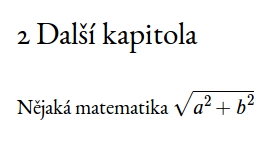
\includegraphics[width=150pt]{examples/scalemathml.png}
  \end{block}
\end{frame}

\begin{frame}
  \frametitle{Jak vložit obálku?}
  \begin{itemize}
    \item Máme dvě možnosti:
      \begin{enumerate}
        \item použít příkaz \texttt{\textbackslash coverimage}
          \begin{itemize}
            \item to vyžaduje explicitní vložení balíčku tex4ebook do dokumentu
            \item obálka se zobrazí v dokumentu
          \end{itemize}
        \item použít příkaz \texttt{\textbackslash CoverMetadata} v konfiguračním souboru
          \begin{itemize}
            \item výhodou je, že nemusíte upravovat dokument
            \item obálka se zobrazí pouze ve čtecí aplikaci
          \end{itemize}
      \end{enumerate}
  \end{itemize}
\end{frame}

\begin{frame}
  \frametitle{Zpracování výstupních souborů}
  \begin{itemize}
    \item výstupní soubory můžeme zpracovat externími příkazy, nebo funkcemi v jazyce Lua
    \item efektivní zpracování umožňují filtry
  \end{itemize}
\end{frame}

\begin{frame}[fragile]
  \frametitle{Příklad pro využití filtrů}
  \begin{verbatim}
    \documentclass{article}
    ...
    \begin{document}
    Co dělat v případě, že se 
    {\bfseries nám nelíbí výstup?}
    \hrule

    Použijeme filtry!
  \end{document}
\end{verbatim}
\end{frame}

\begin{frame}[fragile]
  \frametitle{Normální výstup má samozřejmě chybnou diakritiku}
\begin{verbatim}
<p class="noindent">Co dělat v případě, že se 
<span class="ecbx-1000">n</span><span 
class="ecbx-1000">ám nel</span><span 
class="ecbx-1000">íb</span><span 
class="ecbx-1000">í v</span><span 
class="ecbx-1000">ýstup?</span>________________________
</p> 
<p class="indent">    Použijeme filtry!
\end{verbatim}
\end{frame}

\begin{frame}[fragile]
  \frametitle{Build soubor s filtry, pokus.mk4}
\begin{verbatim}
local filter = require "make4ht-filter"
local process = filter{"cleanspan", "hruletohr"}
Make:htlatex()
Make:htlatex()
Make:match("html$",process)
Make:match("html$",
"tidy -m -utf8 -asxhtml -q -i ${filename}")
\end{verbatim}
\end{frame}

\begin{frame}[fragile]
  \frametitle{Vyčištěné HTML}
\begin{verbatim}
<body>
<p class="noindent">Co dělat v případě, že se 
<span class= "ecbx-1000">nám nelíbí výstup?
</span>
</p>
<hr class="hrule" />

<p class="indent">Použijeme filtry!</p>
</body>
\end{verbatim}
\end{frame}

\begin{frame}
  \frametitle{EDUPUB}
  \begin{itemize}
    \item profil pro ePUB 3 určený pro vzdělávací materiály
    \item \url{http://www.idpf.org/epub/profiles/edu/spec/}
    \item přidává sémantická metadata 
  \end{itemize}
\end{frame} 

\begin{frame}
  \frametitle{Příklad konfigurace vlastního balíčku: EDUPUB}
  \begin{itemize}
    \item vytvoříme balíček pro vkládání učitelských poznámek
    \item poznámky se vypíšou pouze učitelům
  \end{itemize}
\end{frame}

\begin{frame}
  \frametitle{Jak toho docílit?}
  \begin{itemize}
    \item balíček bude mít volitelný argument \texttt{teacher}
    \item učitelské poznámky se vypíšou pouze pokud je balíček vložen s tímto argumentem
    \item dva řídící soubory obsahující kompletní preamble, vkládají TeXový 
      soubor, který je pro učitele i studenty stejný
  \end{itemize}
\end{frame}

\begin{frame}[fragile]
  \frametitle{Řídící soubor pro učitele: teacher.tex}
\begin{verbatim}
\documentclass{article}
...
\usepackage[teacher]{edupub}
\begin{document}
\newcommand\odpoved[1]{\\ \teacherinfo{#1}}
\begin{enumerate}
\item Jak se jmenuje náš největší had?\odpoved{Užovka stromová}
\end{enumerate}

\end{document}
\end{verbatim}
\end{frame}

\begin{frame}[fragile]
  \frametitle{Řídící soubor pro studenty: student.tex}
\begin{verbatim}
\documentclass{article}
...
\usepackage[]{edupub}
\begin{document}
\newcommand\odpoved[1]{\\ \teacherinfo{#1}}
\begin{enumerate}
\item Jak se jmenuje náš největší had?\odpoved{Užovka stromová}
\end{enumerate}

\end{document}
\end{verbatim}
\end{frame}

\begin{frame}[fragile]
  \frametitle{TeXový soubor text.tex}
\begin{verbatim}
\newcommand\odpoved[1]{\\ \teacherinfo{#1}}
\begin{enumerate}
\item Jak se jmenuje náš největší had?
\odpoved{Užovka stromová}
\end{enumerate}
\end{verbatim}
\end{frame}


\begin{frame}[fragile]
  \frametitle{balíček edupub.sty}
\begin{verbatim}
\ProvidesPackage{edupub}
\RequirePackage{kvoptions}
\RequirePackage{etoolbox}
\newbool{teacher}
\boolfalse{teacher}
\newcommand\teacherinfo[1]{}
\DeclareVoidOption{teacher}{%
  \renewcommand\teacherinfo[1]{%
    \edupub@print@teacherinfo{##1}}
  \booltrue{teacher}}
\newcommand\edupub@print@teacherinfo[1]{#1}
\ProcessKeyvalOptions*
\end{verbatim}
\end{frame}

\begin{frame}[fragile]
  \frametitle{konfigurace pro balíček edupub, edupub.4ht}
\begin{verbatim}
\ifbool{teacher}{%
  \Configure{OpfMetadata}
  {\HCode{<dc:type>teacher-edition</dc:type>}}
}{}%
\end{verbatim}
\end{frame}

\begin{frame}[fragile]
  \frametitle{konfigurace pro balíček edupub, edupub.4ht}
\begin{verbatim}
\NewConfigure{teacherinfo}{2}

\let\old:teacherinfo\edupub@print@teacherinfo

\renewcommand\edupub@print@teacherinfo[1]{
  \a:teacherinfo
  \old:teacherinfo{#1}
  \b:teacherinfo
}
\Configure{teacherinfo}
{\HCode{<span epub:type="answer">}}
{\HCode{</span>}}
\end{verbatim}
\end{frame}

\begin{frame}[fragile]
\frametitle{A výsledek?}
\begin{block}{student}
\begin{verbatim}
<li   class="enumerate" id="x1-3x1">
Jak se jmenuje náš největší had?<br 
class="newline" /></li>
\end{verbatim}
\end{block}
\begin{block}{učitel}
\begin{verbatim}
<li    class="enumerate" id="x1-3x1">
Jak se jmenuje náš největší had?<br 
class="newline" /> 
<span epub:type="answer">Užovka stromová </span> 
</li>
\end{verbatim}
\end{block}
\end{frame}


\begin{frame}
\frametitle{To je vše}
\begin{block}{}
Děkuji za pozornost
\end{block}
\end{frame}

\end{document}
